\documentclass[../thesis.tex]{subfiles}
\begin{document}
\chapter{Examination of Trading Algorithms}
\label{ch:tradingalgos}

In this chapter we examine numerous algorithmic trading methods. We discuss stock trading terms and data before moving into different momentum based strategies followed by a discussion on pairs trading. Chapter~\ref{ch:experimentsalgos} examines the effectiveness of these strategies discussed below. 

\section{Stock Trading and Data}
\label{stocktradingdata}
 
We use Quandl, a financial data platform, to obtain the different stock ticker data. Specifically, we used the \textit{WIKI} and \textit{AS500} datasets to acquire stock data. The former contains end-of-day stock pricing data while the latter contains intraday data, with updated pricing for each minute in a day of trading. While these datasets include numerous stock statistics, such as volume and adjusted price metrics, we only consider closing price for both of our datasets. The stocks used in all strategies are found in Figure~\ref{stocktable}. These stocks were chosen given the availability of NASDAQ and S\&P500 stocks in the Quandl dataset and cover a variety of industries. This is important because we need to account for different performances of stocks across multiple industries. Certain large tech stocks like \texttt{FB} or \texttt{GOOG} have had incredible trajectories and performances whereas other stocks outside of the tech industry like \texttt{HAS}, have performed more moderately. The range of stocks chosen encompass nearly all of the major industries throughout the world.

\begin{figure}[h]
\centering
\includegraphics[width=85mm]{stock_table.png}
\caption{Table of stocks used in our study \label{overflow}}
\label{stocktable}
\end{figure}


\textit {Buy} and \textit {sell signals} are used throughout the study. Algorithms can generate a variety of buy and sell signals at a specific point in time, indicating that a denomination of stocks should be purchased or sold at that specific point in time. The strategies use closing price data from October 1st, 2006 to January 1st, 2017. Some strategies use intra-day stock data, which is minute-by-minute data of stock prices from October 26, 2018. Other additional terms need to be defined. \textit {Securities} and \textit{stocks} are used interchangeably throughout the paper and effectively have the same meaning. Specifically, securities have more of a broad definition, as securities include stocks, bonds, mortgages, and others. When discussing how stocks will move in the future, we use \textit {bearish signals} to signal trends of downturn and \textit {bullish signals} for positive, upward trends \cite{Aldridge2010}. 

Graphs can be interpreted as follows. Figure~\ref{SMAfigure} shows the "Golden Cross" strategy applied to \texttt{AAPL}. Purple triangles, which are angled upwards, are buy signals while black triangles angled downwards are sell signals. After about 400 days through the trading period, the strategy generated a buy signal, as denoted by the purple triangle. At about 500 days through the trading period, the following sell signal was generated. This generated a profit of almost \$20 per share for this specific instance. The orange line is the long moving average, the blue line is the short moving average, and the red line gives the price of \texttt{AAPL}. 

\begin{figure}[h]
\centering
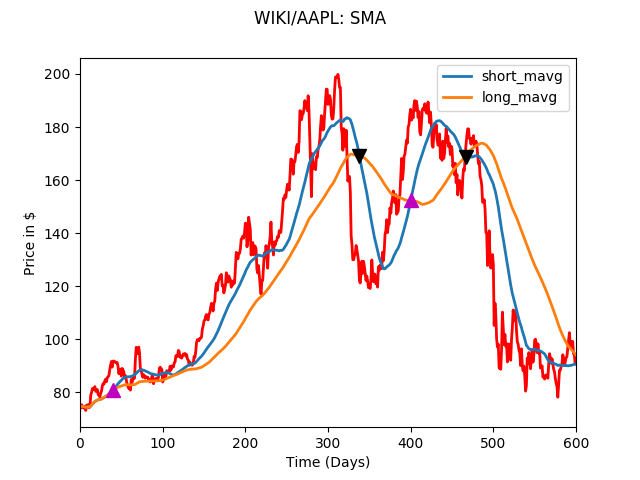
\includegraphics[width=90mm]{AAPLsma.png}
\caption{Simple Moving Average - "Golden Cross" Strategy applied to \texttt{AAPL} \label{overflow}}
\label{SMAfigure}
\end{figure}


\section{Momentum Trading Strategies}

Momentum indicators are AT tools used to measure the recent performance, or momentum, of a stock \cite{Chong2014}. In this section, we examine trading strategies that leverage different momentum indicators to generate optimal buy and sell signals.

\subsection{Simple Moving Average}
Simple Moving Average (SMA) is an elementary AT measure. It is mostly used to measure average stock price over a period of time, however certain strategies solely rely on SMA. It looks at a rolling average of a specified window. Mathematically this can be defined as \cite{AlmeidaTeixeira}:  \[ SMA(t) = 1/n \sum_{i=t-n}^{t}x(i) \]  In words, this gets the average price over a specified window of time for a specified function. In the context of the stock market, SMA can be applied for both short term and long term averages, with the former under an hour while the latter can be hundreds of days or more. In application to the stock market and closing prices, this creates an average closing price for a specified amount of time, which gives an indicator of price swings in that period of time.

SMA is commonly leveraged into a strategy that uses a dual moving average, also known as the "Golden Cross" \cite{AlmeidaTeixeira}. It works by taking two different SMA's - a short window and a long window. In our implementation, we chose a 40-day window and 200-day window, giving insight into a strategy that uses longer averages. The short window crossing below the long window gives a buy signal reinforced by high trading volumes. The long window crossing below the short window is considered bearish and gives a sell signal, as this signals that the stock is currently overvalued and will devalue. As demonstrated in Figure~\ref{SMAfigure}, the strategy generates about 30 buy or sell signals over the period tested.

\subsection{Expected Moving Average}

Expected Moving Average (EMA) is closely linked to SMA. Like SMA, EMA functions over a rolling window; however, it is calculated differently. Mathematically, EMA is calculated with $F_i$ = the value associated with the moving average at period zero, $\alpha$ = smoothing constant, and $X_i$ = closing price of the security at period $i$ \cite{James1968}:  \[F_i = F_{i-1} +\alpha(X_i - F_{i-1})\]  In words, the EMA is found by multiplying the closing price subtracted by the EMA from the previous day times a multiplier plus that prior day's average. This makes this measure far more weighted towards recent prices than SMA.

Like our implementation of SMA, EMA is commonly implemented with dual high and low value average. It takes two different EMA's, one with a low window and the second with a high window. However, because EMA reacts more closely to recent stock prices shorter windows are more commonly chosen. For our implementation, 12-day and 26-day windows were used. The short window crossing below the long window gives a buy signal reinforced by high trading volumes while the opposite is considered bearish and gives a sell signal. Figure~\ref{EMAfigure} demonstrates the EMA trading strategy applied to \texttt{AAPL}. Because smaller windows are used than our SMA implementation, we see far more frequent buy and sell signals. Additionally, we see the short and long expected moving average lines follow the price line far closer than the SMA implementation.

\begin{figure}[h]
\centering
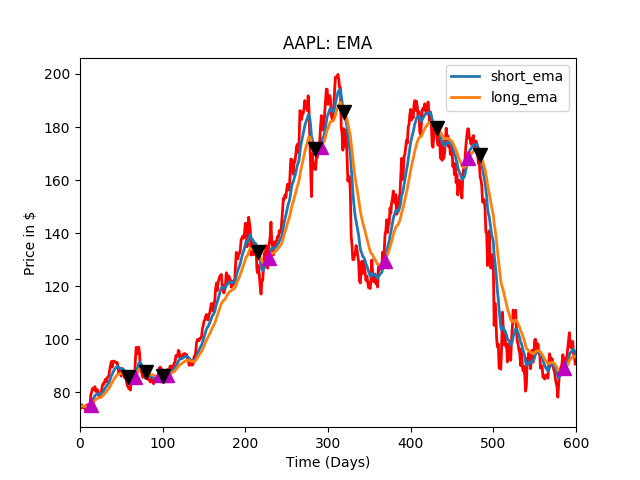
\includegraphics[width=90mm]{AAPLema.png}
\caption{Dual Moving Average Strategy with Exponential effects applied to \texttt{AAPL} \label{overflow}}
\label{EMAfigure}
\end{figure}

\subsection{Bollinger Bands}

Bollinger Bands were introduced by John Bollinger in the 1980s \cite{Liu2006}. This strategy uses three bands, with the two outer bands derived from a standard deviation of the moving average. They provide a relative definition for high and low stock prices. Just like the previously examined techniques, the method uses a moving average as its basis, but instead incorporates 3 different bands separated by standard deviation. Because of this use of standard deviation, which is determined by market volatility, Bollinger Bands adjust themselves to market conditions. Precisely, the bands are calculated as follows with M - Middle Band, U - Upper Band, L - Lower Band, STD(x) - standard deviation of period x: \[M = SMA(12), U = M + 2 * STD(12),  L = M - 2 * STD(12)\] When the market is more volatile the bands widen and when the market becomes less erratic, the bands move closer together \cite{Liu2006}. Unlike the previous techniques, this strategy uses market conditions to evaluate trading orders.

This strategy is implemented with these 3 bands as mentioned above. For our implementation, a 12 day window was chosen to test out the algorithm, as this has been proven to be the most effective \cite{Liu2006}. When the closing price drops below the lower band, this gives a buy signal, as once a lower band has been broken due to heavy selling, the stock price will revert back and head towards the middle band. The opposite is true for when the closing price breaks the upper band, as this is indicative of heavy buying. The closing price approaching the upper band gives a bearish signal while approaching the lower band gives a bullish signal.  This strategy is showing in Figure~\ref{BBANDSfigure}. This measure can generate multiple buy or sell signals in a row. Looking at the range of days between 150 and 250, six straight sell signals are generated. In the range of days between 400 and 500, many buy signals are generated. Both of these trends are indicative of the market giving only bearish or bullish indicators stemming from the use of standard deviation measuring the volatility of price conditions.

\begin{figure}[h]
\centering
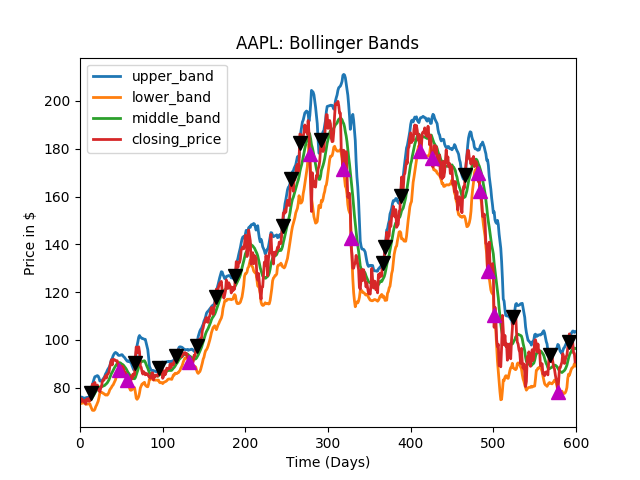
\includegraphics[width=90mm]{AAPLbbands.png}
\caption{Bollinger Bands strategy applied to \texttt{AAPL}  \label{overflow}}
\label{BBANDSfigure}
\end{figure}

\subsection{RSI - Relative Strength Index}

Relative Strength Index (RSI) is a momentum indicator that measures the magnitudes of price changes to analyze overbought or oversold stocks. It demonstrates a particular security's recent performance over a relatively short window compared to the mean. This indicator is widely used today in algorithmic trading. The measure is a value between 0 and 100 at a specific date. The equation for RSI is as follows with $RS$ defined as average gain of up periods divided by the average gain of down periods over a specified window $x$ \cite{Chong2014}: \[RSI = 100.0 - (100.0 / (1.0 + RS(x))\] Therefore, a large RSI value is indicative of stocks that have had recent larger gains compared to losses while a low RSI value is indicative of stocks with poor recent performance compared to the mean.

This strategy takes advantage of mean reversion. Our implementation uses a very simple method. Sell signals are generated when the RSI is over 70 and buy signals are generated when the RSI is under 30 \cite{Chong2014}. This is very logical, as expected gains are the largest when a stock has performed poorly recently and is expected to revert back to the mean. This strategy also uses a 14 day window, which is standard across the industry. Figure~\ref{RSIfigure} shows this strategy when run on \texttt{AAPL}. The second subfigure generates the buy and sell signals, as it shows the RSI of the stock throughout the period tested. These signals generated from the second subfigure are then plotted on the first subfigure over the stock price. Clearly, this strategy generates a large quantity of trading signals over the period.

\begin{figure}[h]
\centering

\begin{subfigure}[t]{0.45\textwidth}
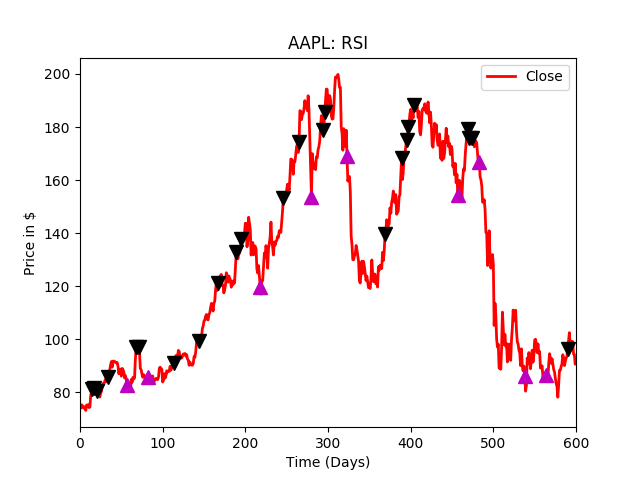
\includegraphics[width=\textwidth]{AAPLrsisignals.png}
\caption{RSI Strategy \label{overflow}}
\end{subfigure}
\begin{subfigure}[t]{0.45\textwidth}
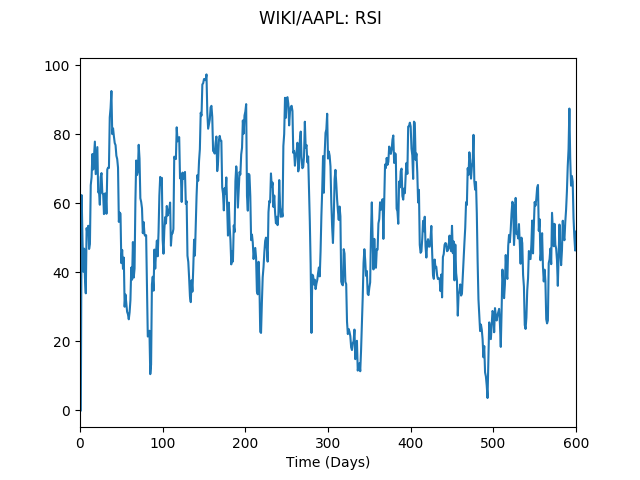
\includegraphics[width=\textwidth]{AAL_RSI.png}
\caption{ RSI of \texttt{AAPL} \label{overflow}}
\end{subfigure}

\caption{RSI strategy applied to \texttt{AAPL}  \label{overflow}}
\label{RSIfigure}
\end{figure}

\subsection{Combining Momentum Indicators - RSI and Moving Average Convergence-Divergence (MACD)}

MACD uses two moving averages to identify trend changes while RSI performs exactly as stated in the above section. The MACD is constructed by subtracting two different sized exponential moving averages from each other. The equation for MACD is as follows and uses $EMA(x)$, with $x$ representing the period in minutes \cite{Chong2014}: \[ MACD = EMA(12) - EMA(16)\] The MACD is then plotted against a signal line, which is defined as S and is the EMA of the 9 minute MACD: \[ S = EMA(MACD(9)) \] Buy and sell signals are then generated by the ``Golden Cross" method. Specifically, this is when the MACD crosses the signal line from below - signaling a momentum swing and a bullish buy signal. A sell signal is the reverse - when the MACD crosses the signal live from above.

Unlike the previously mentioned strategies, this one combines indicators to generate more robust trading signals. Because there are two different measures working at the same time, buy signals are generated by both the RSI and MACD measures giving bullish signals within 3 minutes of each other. Sell signals are generated by either one of the measures producing a sell. Under this strategy, buy signals are very rarely generated while either strategy generating a sell denotes all shares to be sold. Because of the selectivity of buy signals, we can expect this technique to be very profitable. This strategy is most effective when run over intra-day data because of the relative infrequency of buy signals, as demonstrated in Figure~\ref{RSIMACDfigure}. Throughout an entire day, only a handful of buy signals were generated. 

\begin{figure}[h]
\centering
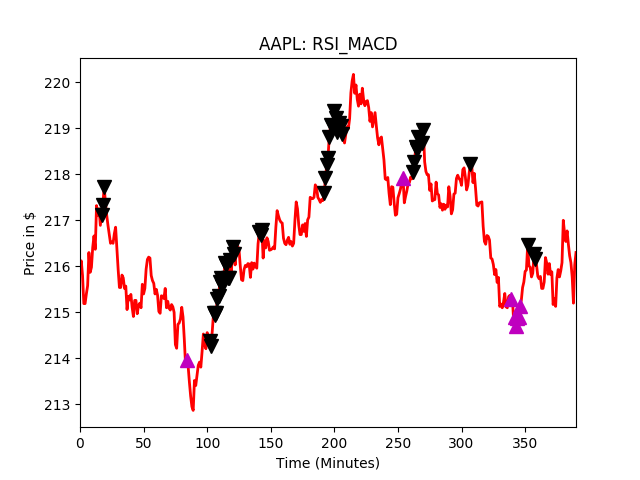
\includegraphics[width=.6\textwidth]{AAPL_RSIxMACD.png}
\caption{RSI and MACD strategy buy and sell signals \label{overflow}}
\label{RSIMACDfigure}
\end{figure}

\section{Pairs Trading - Arbitrage and Mean Reversion}

Pairs trading is an AT strategy that chooses two economically linked stocks and profits off the divergence in spread of prices. Pairs trading takes advantage of statistical arbitrage, which is attempted profit from pricing inefficiencies identified through mathematical models. The most basic assumption is that prices will move towards their historical average, known as mean reversion. However, unlike other instances of mean-reversion, this strategy has a distinct advantage of always being hedged against market movements \cite{Fu2009}. 

A challenge with pairs trading is choosing pairs of stocks that have related performances. Often when given two stocks that are linked economically (i.e. Pepsi and Coca-Cola), we expect the spread to remain relatively constant over time. However, there might be divergence in the spread between these two pairs cause by factors such as supply/demand changes or changes in volume in a particular stock.  Another problem with this is finding stocks that are closely related. Because we need to have stocks that behave similarly, we use \textit{cointegration} to identify pairs of similarly behaving stocks. 

Cointegration is a stationary measure that highlights horizontal trends \cite{Gatev2006}. Unlike correlation, which only tracks similarly moving magnitudes over time, it instead tells how the difference between two regression lines changes over time. Our implementation uses the Python extension \texttt{statsmodels} to generate the p-value for cointegration. It is absolutely key to have related stocks, as this strategy takes advantage of mean reversion. In other words, we expect stocks to revert back to their original mean in relation to other similarly behaving ones. Now this is quite difficult, as it is hard to find stocks that behave very similarly. After running comparisons of cointegration, certain tech stocks such as \texttt{INTC} and \texttt{MFST} were found to behave similarly. We tested cointegration for all combinations of stocks tested and only found five satisfactory combinations: \texttt{QCOM/SBUX, INTC/MSFT, AMD/SBUX, AMD/EBAY, AMD/VOD}. 

To generate trading signals, a Zscore is generated from the ratio of prices R(i) = ClosingPriceStockX/ClosingPriceStockY on a particular day $i$, the overall mean of ratio of prices M = AVG(R), and the standard deviation of the price ratio STD = STD(R): \[ Z = (R(i) - M)/STD\] The Zscore is a measure of how far away the current ratio of prices is away from its mean. Figure~\ref{PAIRSfigure}b shows the Zscore of both \texttt{INTC} and \texttt{MSFT}. Because of mean reversion, we can use this as a good indicator for buy and sell signals. A buy signal is generated when the zscore drops below negative one, as we expect the zscore to return to its mean of zero. A sell signal is generated when the zscore goes above one, as the stock is currently overvalued because we expect the stock to return to its mean of zero \cite{Fu2009}. These thresholds are shown in Figure~\ref{PAIRSfigure}b. In context of the pair of stocks, on buy signals the first stock in the pair is bought while the second is sold or shorted. The reverse is true on sell signals. Figure~\ref{PAIRSfigure}a shows this strategy applied to \texttt{INTC} and \texttt{MSFT}. Each time a buy signal is generated at a particular day the other stock has a matching sell signal and vice versa.

\begin{figure}[h]
\centering
\begin{subfigure}[t]{0.48\textwidth}
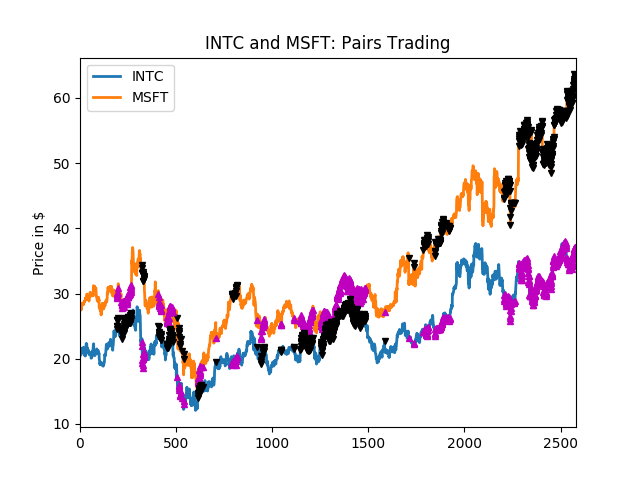
\includegraphics[width=\textwidth]{Intc_msft_signals.png}
\caption{Pairs Trading Strategy  \label{overflow}}
\end{subfigure}
\begin{subfigure}[t]{0.48\textwidth}
\includegraphics[width=\textwidth]{zscore.png}
\caption{Zscore of INTC and  MSFT \label{overflow}}
\end{subfigure}

\caption{Pairs Trading strategy applied to INTC and MSFT  \label{overflow}}
\label{PAIRSfigure}
\end{figure}

\end{document}
